\documentclass[12pt,a4paper]{report}
\usepackage[utf8]{inputenc}
\usepackage{amsmath}
\usepackage{amsfonts}
\usepackage{amssymb}
\usepackage{graphicx}
\usepackage{commath}
\usepackage{array}
\usepackage{tabularx}
\usepackage{latexsym}
\usepackage[italian]{babel}
\usepackage{url} 
\usepackage{hyperref}
\usepackage[nottoc]{tocbibind}	
\usepackage[a4paper,top=1.5cm,bottom=1.8cm,left=1.5cm,right=1.5cm]{geometry}
\graphicspath{ {images/} }
\begin{document}
	\begin{titlepage}
		\begin{center}
	\huge{\textbf{Università della Calabria}}
	\begin{figure}[tb]
		\centering
		
\includegraphics[scale=0.5]{logoUNICAL}
	\end{figure}
\end{center}
\begin{center}
	\line(1,0){400}\\[5mm]
	\Large{\textbf{Dipartimento di Matematica e Informatica}}
	\\\Large{\textbf{Corso di laurea in Informatica}}
	\\\vfill
	\Huge{\textbf{Data Warehouse Project \\\noindent CORDIS - EU research 2007-2013}}
	\vfill
\end{center}
\vfill
	\noindent \hfill  \Large{\text{Giovanni Brunetti}} \par
	\noindent \hfill	\Large{\textit{Matricola:}\text{193452}}
	\begin{center}
	\line(1,0){400}\\[5mm]
	{\large{\bf Anno accademico 2017/2018}}\\
\end{center}

	\end{titlepage}
	\section*{Introduzione}
	Lo scopo del progetto è quello di costruire un sistema di Data Warehouse basato sui dati relativi all'assegnazione di progetti scientifici da parte dell'UE alle varie organizzazioni mondiali.\\\noindent
	Per far ciò si provvederà alla creazione del/dei data-mart necessari per i fatti di interesse in modo da permettere lo svolgersi delle analisi OLAP su di essi.
	La progettazione ha seguito le varie fasi relativi all'approccio \textbf{source oriented}, includendo lo studio delle sorgenti, comprendendo operazioni di pulizia e di trasformazione dei dati per comprendere i dati ed il dominio di interesse. In seguito si è passato alla fase di alimentazione del database e dello studio dei dati ottenuti tramite analisi.\\\\\noindent
	Per la fase di studio ,di ETL ed alimentazione del DB si è utilizzato il software Pentaho, mentre per lo studio dei dati e l'effettuazione delle analisi si è utilizzato il software Tableau.
	\section*{Sorgente dei dati}
	La sorgente dei dati è reperibile all' url  "https://data.europa.eu/euodp/data/dataset/cordisfp7projects" sotto forma di file csv.\\\noindent
	La sorgente è composta da 6 file, essi contengono tutte le informazioni relativi ad ogni singolo progetto assegnato dal 2013 al 2017. La prima fase del progetto si è dunque concentrata nello studio di tutti i file per capire come essi erano connessi tra di loro. Essi infatti presentavano molte ripetizioni di attributi nei diversi file.
	Per ciascuna delle assegnazioni le principali informazioni espresse e rilevanti del il data mart sono:
	\begin{itemize}
		\item nome del progetto;
		\item le organizzazioni coinvolte nel progetto;
		\item la nazionalità di ogni organizzaione;
		\item programma di appartenenza del progettto;
		\item contributo economico dell'ue per ogni organizzazione;
		\item data di inizio e di fine.
	\end{itemize}
\section*{Architettura di sistema}
L'architettura di sistema scelta per l'implementazione è quella a 3 livelli. Questa scelta è dovuta al fatto di avere più file come sorgente. Il secondo livello, ovvero quello dei dati riconciliati, permette di integrare le molteplici sorgenti per definire un unica fonte di dati operazionali. Così facendo si divide la fase di pulitura e di \textbf{ETL}, con la conseguente creazione delle dipendenze funzionali, da quello dell'alimentazione del Data Warehouse.
\begin{figure}[htbp]
	\centering
	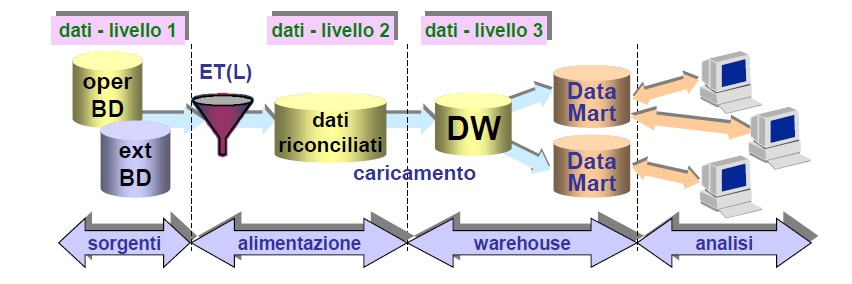
\includegraphics[scale=0.6]{architettura}
\end{figure}
\section*{Database riconciliato}
Per la creazione del livello riconciliato è stato utilizzato un modello E/R. Prima di ciò è stato effetuta la fase di \textbf{Ricognizione} sul dominio applicativo per costruire le dipendenze funzionali tra i dati iniziali. Lo schema E/R ottenuto è il seguente:\\
\begin{figure}[htbp]
	\centering
	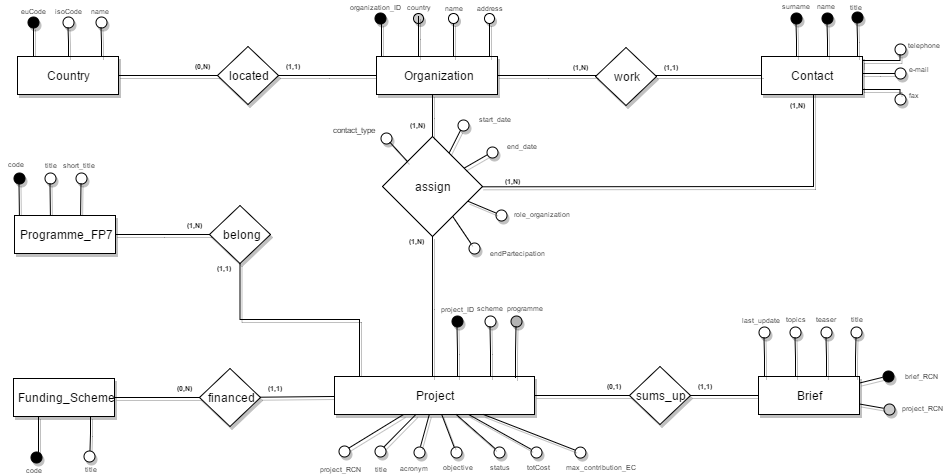
\includegraphics[scale=0.50]{reconciled}
\end{figure}
\\Come si può subito notare il fatto di interesse (\textbf{Data Mart}) è quello relativo all'assegnazione dei progetti, \textbf{assign}.
\section*{Progettazione Concettuale}
La prima fase per la progettazione concettuale di un data mart è quello di definire il fatto di interesse, cioè il concetto primario su cui verranno fatte tutte le analisi e le operazioni. Come già detto in precedenza il fatto scelto in questo progetto è l'assegnazione vera e propria del progetto. 
Si costruisce così l'\textbf{albero degli attributi}, attraverso il
quale, partendo dal fatto come radice, si delimita l'area di interesse dello schema inserendo come figli tutte le dipendenze funzionali in modo ricorsivo.
\begin{figure}[htbp]
	\centering
	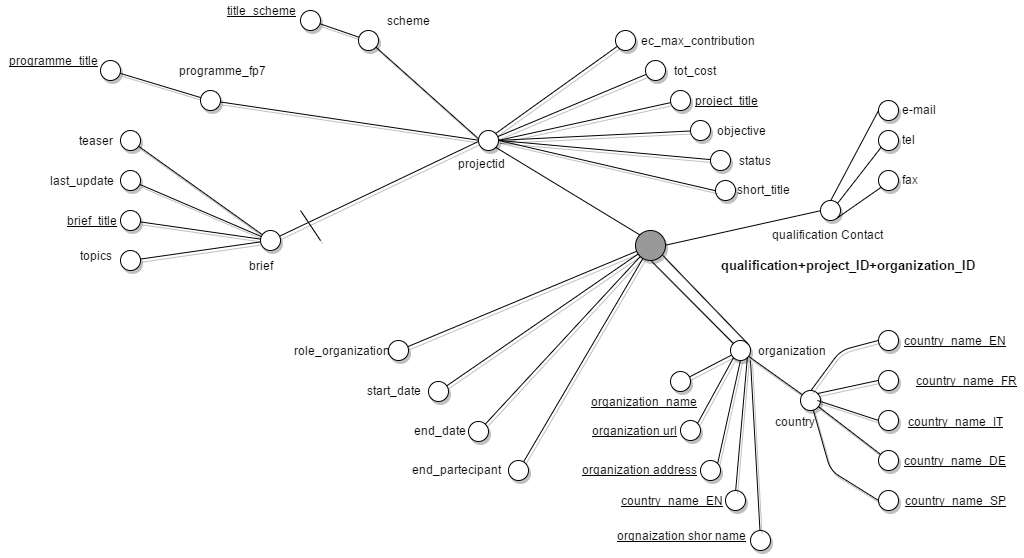
\includegraphics[scale=0.40]{attribute-tree}
\end{figure}
\\In seguito l'albero viene ristrutturato tramite pruning, operazioni sulle dipendendenze funzionali (potatura e innesto) ed eliminando gli attributi irrilevanti ai fini dell'analisi.
\begin{figure}[htbp]
	\centering
	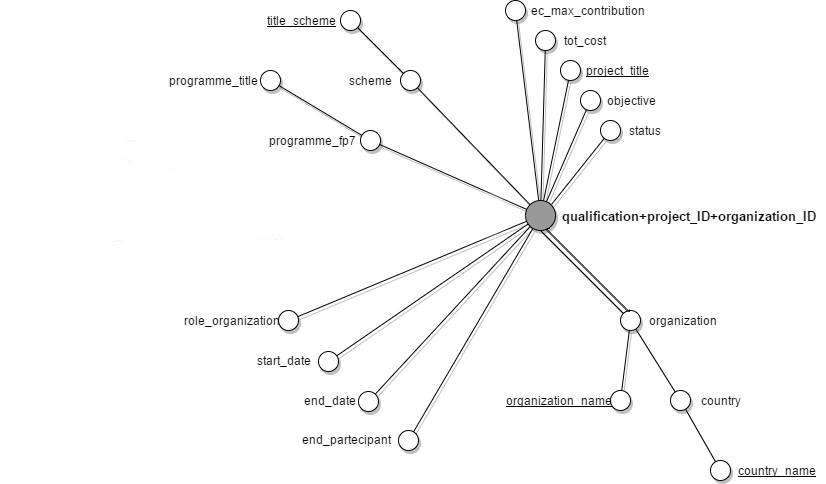
\includegraphics[scale=0.40]{attribute-tree-final}
\end{figure}
\\Le operazioni effettuate sono le seguenti:
\begin{itemize}
	\item pruning del ramo brief e qualification, in quanto irrilevante per le analisi;
	\item innesto del solo qualificatore qualification in assign;
	\item potatura attributi insignificanti per le analisi (solo descrittivi o insignificanti);
	\item innesto attributi del sotto albero project direttamente al fatto assign.
\end{itemize}
\vspace*{1cm}
Una volta ottenuto l'albero degli attributi si passa alla definizioni delle \textbf{dimensioni}, le quali permetteranno l'aggregazione degli eventi, e delle \textbf{misure}, che di fatto definiscono dei criteri di valutazione del fatto.
Le dimensioni scelte sono programme, organization e start\underline{ }date e end\underline{ }date.
\\\noindent Con la definizione di misure e dimensioni si può passare alla creazione dello \textbf{schema di fatto}, composto dal fatto centrale, con le misure al suo interno, e dalle \textbf{gerarchie}, che corrispondono ai rami dell'albero degli attributi aventi come radice una dimensione.
\vspace*{2cm}
\\Durante questa fase si è potuto applicare nuove operazioni di modifica, quali potatura e innesto. Si è effettuato l'innesto degli attributi year, month e day alle dimensioni date (start e end). Per comodità è stata usata la stessa radice per start e end, poiché avevano una gerarchia condivisa. Inoltre per facilità di aggregazione, project è stato riinnestato come dimensione, per permettere un'analisi per singolo progetto in modo più semplificato.
\begin{figure}[htbp]
	\centering
	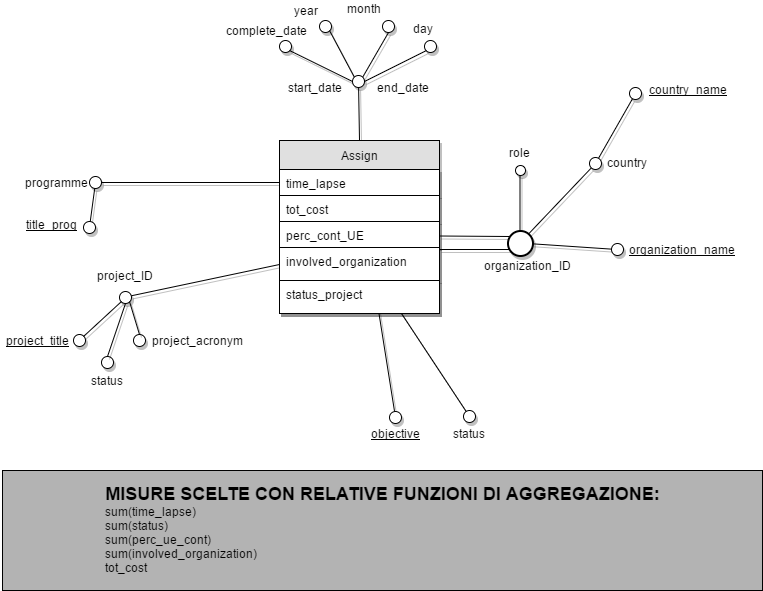
\includegraphics[scale=0.70]{Fact_Scheme}
\end{figure}
\newpage\noindent
Una volta creato il fact model non resta che creare lo \textbf{star\underline{ }schema}, che altro non è che la rappresentazione, attraverso tabelle dello stesso fact model. Si costruisce 
\begin{figure}[htbp]
	\centering
	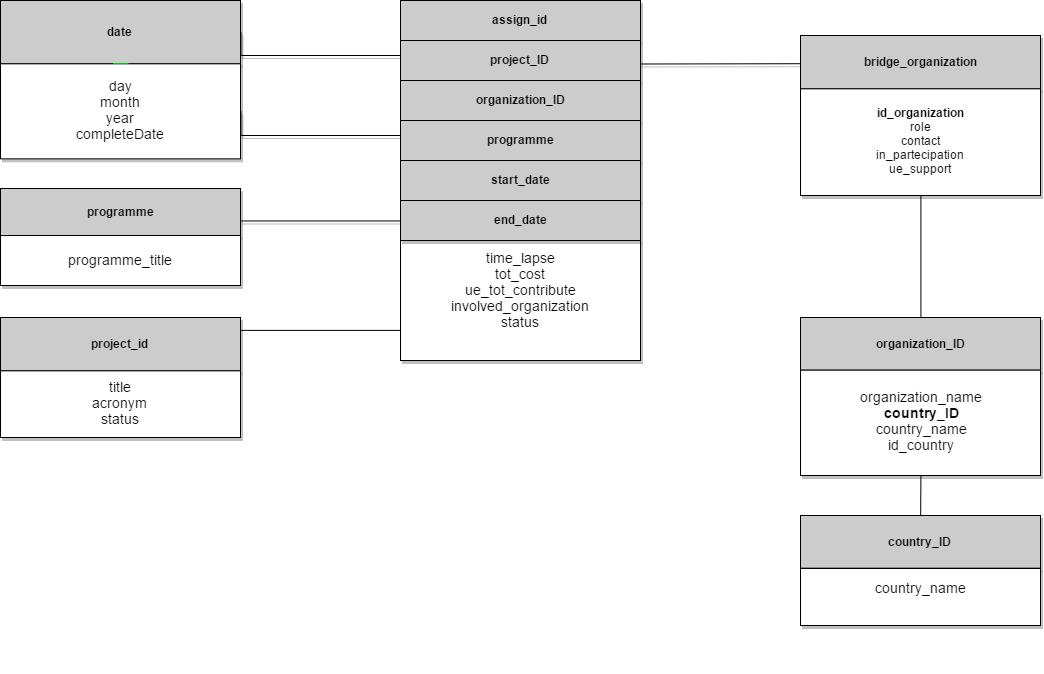
\includegraphics[scale=0.50]{star_scheme}
\end{figure}
\\\\\noindent
Si noti che è stato necessario la gestione dell'\textbf{arco multiplo} tra la dimensione organization e il fatto. Ciò è stato risolto con l'inserimento di una \textbf{bridge\underline{ }table}.\\\noindent
Si è scelto di utilizzare questo approccio, invece che uno \textbf{push\underline{ }down}, in modo da non duplicare istanze all'interno della fact table e risparmiare dunque memoria. Infatti il metodo push\underline{ }down consisteva nell'inserire più eventi con le combinazioni dell'attributo multiplo all'interno del fatto stesso.\\\noindent Nonostante sia vero che il metodo push down garantirebbe una maggiore velocità, il metodo della bridge\underline{ }table garantisce una maggiore facilità nelle analisi d'impatto.
\section*{Alimentazione}
L'alimentazione del Data Warehouse è avvenuto basandosi sul riconciliato. Infatti si è fatto in modo che le operazioni di modifica e di aggiornamento possano avvenire solo all'interno del riconciliato.
\\\\
\noindent Per far ciò si sono utilizzati dei dati temporali per verificare l'eventuale modifica (campo \textbf{last\underline{ }update}) delle tuple. Ciò è bastato in quanto le dimensioni appartengono tutte a \textbf{Slowly Changing di Tipo 1}, in cui non vi è bisogno di tenere traccia dei precedenti valori dei campi aggiornati, ma solo l'ultima versione.
\\\\\noindent
L'alimentazione di Data warehouse avviene dunque tramite \textbf{ETL-update} ed \textbf{ETL-refresh}. Il primo consiste nell'effettuare l'aggiornamento dei dati in modo periodico, ad esempio settimanalmente, prelevando i dati dal database riconciliato.\\
Il secondo invece consiste nel caricamento dei dati in modo statico quando il data warehouse è vuoto.\newpage
\section*{Analisi effettuate}
Si sono effettuate le seguenti analisi per capire la partecipazione delle varie organizzazioni e prelevare informazioni dai progetti:
\begin{itemize}
	\item Dashboard generale relativa ad una singola organizzazione;
	\item Dashboard generale relativa all'insieme delle organizzazioni di una o più nazioni;
	\item Varie analisi singole sulle organizzazioni o su gruppi di organizzazioni;
	\item Dashboard generale relativa ad una singola nazione o un sottoinsieme di essi;
	\item Varie analisi sulle organizzazioni;
	\item Visuale su mappa dell'impegno delle singole nazioni;
	\item Dashboard generale relativa ai progetti, con possibilità di filtro su uno solo o più;
	\item Varie analisi sui progetti, quali media fondi, tempo previsto ecc;
	\item Dashboard generale basata sul tempo, dunque su data di assegnazione e di chiusura per verificare il trend temporale;
\end{itemize}
Sulla maggior parte delle analisi è possibile applicare determinati filtri per restringere le analisi in un lasso di tempo, a determinate nazioni o ad un certo valore. Ad esempio potremmo essere intenzionati ad analizzare tutte le nazioni che hanno preso parte a più di 100 progetti nell'arco temporale dal 2012 al 2013.
\end{document}